% =====================================================================
% main.tex — Documento Principal (Modular)
%
% Autor: Gabriel Omar Murillo Medina
% Universidad de las Fuerzas Armadas — ESPE
% Ingeniería en Software
%
% Compilar: pdflatex main.tex (x2 para referencias cruzadas)
% =====================================================================

\documentclass[10pt,journal,compsoc]{IEEEtran}

% --- Preámbulo modular ---
% ==========================================
% PREÁMBULO DEL DOCUMENTO
% Configuración, paquetes y estilos
% ==========================================

\usepackage[utf8]{inputenc}
\usepackage[english]{babel}
\usepackage{amsmath,amsfonts,amssymb}
\usepackage{booktabs}
\usepackage{graphicx}
\usepackage{multirow}

% --- Configuración de Tipografía ---
% Usamos lmodern en su variante Sans-Serif para un aspecto ultra-moderno, limpio y de vanguardia (Fintech/HFT)
\usepackage{lmodern}
\renewcommand{\familydefault}{\sfdefault}
\usepackage[T1]{fontenc}
\usepackage{microtype} % Mejora el espaciado y justificación

% --- TikZ y PGFPlots ---
\usepackage{tikz}
\usepackage{pgfplots}
\pgfplotsset{compat=1.18}
\usetikzlibrary{shapes.geometric, arrows.meta, positioning, fit, calc, backgrounds, shadows, decorations.pathreplacing}

% Paleta de colores profesional (Inspirada en paletas HFT/Fintech)
\definecolor{techblue}{RGB}{10, 50, 120}
\definecolor{neoncyan}{RGB}{0, 200, 255}
\definecolor{alertred}{RGB}{220, 20, 60}
\definecolor{hotgreen}{RGB}{0, 180, 80}
\definecolor{coldblue}{RGB}{100, 150, 250}

% Configuración global de PGFPlots para gráficos más modernos
\pgfplotsset{
    modern chart/.style={
        ybar,
        bar width=22pt,
        enlarge x limits=0.25,
        width=\linewidth,
        height=6.5cm,
        axis line style={opacity=0}, % Oculta los bordes feos
        major grid style={dashed, gray!30},
        ymajorgrids=true,
        xmajorgrids=false,
        tickwidth=0pt,
        nodes near coords,
        nodes near coords align={vertical},
        nodes near coords style={font=\bfseries\small},
        legend style={
            at={(0.5,-0.2)},
            anchor=north,
            legend columns=-1,
            draw=none, % Sin borde en la leyenda
            fill=white!80
        },
        label style={font=\bfseries},
        tick label style={font=\small}
    }
}

% --- Estilos de Código (Listings) ---
\usepackage{listings}
\usepackage{xcolor}

\definecolor{codegreen}{rgb}{0,0.6,0}
\definecolor{codegray}{rgb}{0.5,0.5,0.5}
\definecolor{codepurple}{rgb}{0.58,0,0.82}
\definecolor{backcolour}{rgb}{0.96,0.96,0.96}

\lstdefinestyle{mystyle}{
    backgroundcolor=\color{backcolour},   
    commentstyle=\color{codegreen}\itshape,
    keywordstyle=\color{techblue}\bfseries,
    numberstyle=\tiny\color{codegray},
    stringstyle=\color{codepurple},
    basicstyle=\ttfamily\footnotesize,
    breakatwhitespace=false,         
    breaklines=true,                 
    captionpos=b,                    
    keepspaces=true,                 
    numbers=left,                    
    numbersep=8pt,                  
    showspaces=false,                
    showstringspaces=false,
    showtabs=false,                  
    tabsize=2,
    frame=leftline,
    framerule=2.5pt,
    rulecolor=\color{techblue!50}
}
\lstset{style=mystyle}

% --- Hyperref ---
\usepackage[colorlinks=true, linkcolor=techblue, citecolor=techblue, urlcolor=techblue]{hyperref}

% --- Balanceo de última página ---
\usepackage{balance}

% --- Espaciado y Ahorro de Espacio para Límite Estricto de 3 Páginas ---
\setlength{\textfloatsep}{6pt plus 2pt minus 2pt}
\setlength{\intextsep}{6pt plus 2pt minus 2pt}
\setlength{\dbltextfloatsep}{6pt plus 2pt minus 2pt}
\setlength{\abovecaptionskip}{3pt plus 1pt minus 1pt}
\setlength{\belowcaptionskip}{2pt plus 1pt minus 1pt}

% Ajuste sutil de listas para evitar saltos huérfanos
\usepackage{enumitem}
\setlist[enumerate]{topsep=2pt, partopsep=0pt, parsep=0pt, itemsep=2pt}
\setlist[itemize]{topsep=2pt, partopsep=0pt, parsep=0pt, itemsep=2pt}


\begin{document}

% --- Metadatos ---
\title{Microarchitectural Dispatch Optimization: Semi-Static Cache-Aware Devirtualization in Ultra-Low Latency C++17}

\author{Gabriel Omar Murillo Medina\\
        \textit{Ingeniería en Software}\\
        \textit{Universidad de las Fuerzas Armadas --- ESPE}\\
        Sangolquí, Ecuador\\
        gomurillo@espe.edu.ec}

\IEEEtitleabstractindextext{%
\begin{abstract}
In High-Frequency Trading (HFT) systems, branch misprediction penalties represent a critical source of non-deterministic latency in the execution critical path. This paper implements and experimentally validates the semi-static conditions technique through \texttt{FastBranch}, a C++17 header-only abstraction that decouples condition evaluation from the critical flow. For multi-threaded concurrent environments, a lock-free and cache-aware scheme is designed, applying cache-line isolation (\texttt{alignas(64)}) and synchronization based on \textit{release/acquire} semantics to mitigate false sharing. Empirical validation on x86-64 hardware with $5\times10^8$ operations using bootstrap resampling statistical analysis ($B=10\,000$) demonstrated a $3.02\times$ speedup (empirical 95\% CI: $[2.90\times, 3.14\times]$, Cohen's $d=1.82$, $p_{\text{boot}} < 0.0001$), reducing latency from 13.81 ns/op to 4.57 ns/op, consistently converging to the branchless theoretical limit (3.90 ns/op). Negative findings are also documented, including performance degradation due to MESI contention in concurrent writer threads.
\end{abstract}

\begin{IEEEkeywords}
Low-Latency Systems, Software Architecture, High-Frequency Trading, Branch Prediction, C++17 Metaprogramming, Cache-Aware Design, Lock-Free Concurrency, Bootstrap Resampling, Performance Evaluation.
\end{IEEEkeywords}}

\maketitle
\IEEEdisplaynontitleabstractindextext
\IEEEpeerreviewmaketitle

% --- Secciones modulares ---
% sec_introduccion.tex
% Section 1: Introduction
\section{Introduction}

\IEEEPARstart{I}{n} the microstructure of electronic financial markets, processing latency constitutes the key differentiating factor between capturing or losing statistical arbitrage opportunities. In High-Frequency Trading (HFT) systems, where opportunity windows are measured in nanoseconds, any source of non-determinism in the execution critical path represents a quantifiable operational risk \cite{bilokon2025}.

Modern processors based on the x86-64 architecture implement 14- to 19-stage super-scalar pipelines with speculative execution. Upon encountering each conditional jump instruction (\texttt{jcc}), the Branch Prediction Unit (BPU) --- typically a TAGE (\textit{Tagged Geometric History Length}) predictor using 2-bit saturating counters --- speculates on the branch outcome before the condition is formally evaluated \cite{intel2012}. A branch misprediction triggers a complete pipeline flush, imposing a deterministic penalty of 13--18 clock cycles \cite{fog2023}.

Bilokon et al. \cite{bilokon2025} propose an architectural solution: \textbf{semi-static conditions}. This technique completely eliminates the conditional jump instruction from the \textit{hot path} using Self-Modifying Code (SMC) or indirect branches, delegating state updates to an asynchronous \textit{cold path}.

The present work pursues four main objectives:
\begin{enumerate}
    \item Quantify the real \textit{speedup} of the semi-static technique over standard \texttt{switch}/\texttt{if-else} control blocks under uniform-random conditions.
    \item Measure the runtime \textit{overhead} of \texttt{std::function} compared to raw function pointers.
    \item Evaluate the multi-threading viability of this pattern.
    \item Identify the boundary conditions where this technique becomes counterproductive.
\end{enumerate}

% sec_metodologia.tex
% Sección 2: Materiales y Métodos
\section{Materiales y Métodos}

\subsection{Diseño Experimental}
Se diseñó un protocolo de validación estadística basado en simulaciones Monte Carlo con $K = 100$ ensayos independientes, cada uno con semilla pseudoaleatoria única generada mediante \texttt{std::random\_device}. Cada ensayo procesó $N = 5 \times 10^6$ operaciones de \textit{dispatch} condicional, totalizando $5 \times 10^8$ observaciones experimentales.

Se evaluaron cuatro estrategias de \textit{dispatch}:
\begin{itemize}
    \item \textbf{\texttt{switch} nativo:} Evaluación condicional en cada iteración (línea base).
    \item \textbf{\texttt{FastBranch}:} Propuesta experimental con punteros crudos y actualización infrecuente ($f_{\text{set}} = 1/1000$).
    \item \textbf{\texttt{FlexBranch}:} Variante con \texttt{std::function} para cuantificar el costo de la abstracción.
    \item \textbf{Control directo:} Llamada sin \textit{dispatch} condicional (límite teórico).
\end{itemize}

Las diferencias se validaron mediante un análisis estadístico no paramétrico de remuestreo (\textit{Bootstrapping}) con $B = 10,000$ iteraciones. Este enfoque permite construir intervalos de confianza (IC) empíricos al 95\%, mitigando las asunciones de normalidad paramétrica que suelen violarse en mediciones de latencia de hardware por interrupciones del SO. Se reporta adicionalmente el tamaño del efecto mediante la $d$ de Cohen.

\subsection{El Problema: Pipeline Flush}

La Fig.~\ref{fig:pipeline} ilustra el mecanismo por el cual una predicción fallida destruye el rendimiento del pipeline superescalar. Cuando el BPU falla, todas las instrucciones ejecutadas especulativamente se descartan, generando una burbuja de 14--18 ciclos.


% El diagrama de pipeline (Fig 1) ha sido trasladado a la discusión para ubicarse en la última página ocupando dos columnas.

\subsection{Implementación y Arquitectura}
Se desarrolló la biblioteca \texttt{semi\_static.hpp} (\textit{header-only}, C++17) con cuatro variantes (Cuadro~\ref{tab:clases}). La arquitectura central se basa en el desacoplamiento físico entre la evaluación de la condición (\textit{cold path}) y la ejecución del \textit{dispatch} (\textit{hot path}), como se ilustra en la Fig.~\ref{fig:arquitectura}.

\begin{table}[ht]
\centering
\caption{Variantes implementadas en \texttt{semi\_static.hpp}}
\label{tab:clases}
\begin{tabular}{@{}lccc@{}}
\toprule
\textbf{Clase} & \textbf{Mecanismo} & \textbf{Heap} & \textbf{Thread-safe} \\ \midrule
\texttt{FastBranch}       & Array \texttt{FuncPtr}   & No & No \\
\texttt{AtomicFastBranch} & Ídem + \texttt{atomic}   & No & Sí \\
\texttt{FlexBranch}       & \texttt{vector<function>} & Sí & No \\
\texttt{AtomicFlexBranch} & Ídem + \texttt{atomic}   & Sí & Sí \\ \bottomrule
\end{tabular}
\end{table}

\setcounter{figure}{1}
\begin{figure}[ht]
\centering
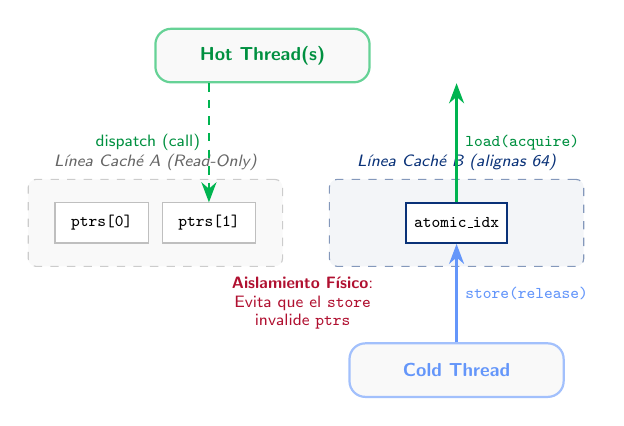
\begin{tikzpicture}[
    scale=0.85, every node/.style={scale=0.85}, % scaled down slightly to fit on 3 pages
    core/.style={rectangle, draw=gray!40, fill=gray!5, thick, rounded corners=2mm, minimum width=3.2cm, minimum height=0.8cm, align=center, font=\footnotesize\bfseries},
    cline/.style={rectangle, draw=gray!40, fill=gray!5, dashed, rounded corners=1mm, minimum width=3.8cm, minimum height=1.3cm},
    cell/.style={rectangle, draw=gray!50, fill=white, minimum width=1.4cm, minimum height=0.6cm, font=\scriptsize\ttfamily},
    arrow/.style={-{Stealth[scale=1.1]}, thick},
]

% Cache Line 1
\node[cline] (line1) at (-2.1, 0) {};
\node[font=\scriptsize\itshape, text=gray!80!black, anchor=south] at (line1.north) {Línea Caché A (Read-Only)};
\node[cell] (p0) at (-2.9, 0) {ptrs[0]};
\node[cell] (p1) at (-1.3, 0) {ptrs[1]};

% Cache Line 2
\node[cline, draw=techblue!50, fill=techblue!5] (line2) at (2.4, 0) {};
\node[font=\scriptsize\itshape, text=techblue, anchor=south] at (line2.north) {Línea Caché B (alignas 64)};
\node[cell, draw=techblue, thick] (idx) at (2.4, 0) {atomic\_idx};

% Threads
\node[core, draw=coldblue!60, text=coldblue] (core0) at (2.4, -2.2) {Cold Thread};
\node[core, draw=hotgreen!60, text=hotgreen!80!black] (core1) at (-0.5, 2.5) {Hot Thread(s)};

% Data flow
\draw[arrow, coldblue] (core0.north) -- (idx.south) node[midway, right, font=\scriptsize\ttfamily, text=coldblue] {store(release)};

\draw[arrow, hotgreen] (idx.north) -- (core1.south-|idx.north) node[midway, right, font=\scriptsize\ttfamily, text=hotgreen!80!black] {load(acquire)};

\draw[-{Stealth[scale=1.1]}, thick, hotgreen, dashed] (core1.south-|p1.north) -- (p1.north) node[midway, left, font=\scriptsize, text=hotgreen!80!black] {dispatch (call)};

% Annotation
\node[font=\scriptsize, text=alertred!80!black, align=center] at (0.1, -1.2) {\textbf{Aislamiento Físico}:\\Evita que el \texttt{store}\\invalide \texttt{ptrs}};

\end{tikzpicture}
\caption{Arquitectura de memoria y sincronización inter-hilo para HFT. La directiva \texttt{alignas(64)} aísla el índice atómico en una línea de caché exclusiva. Esto previene que las actualizaciones del \textit{Cold Thread} invaliden el caché L1 de los punteros a función (\textit{false sharing}). La semántica \textit{release/acquire} garantiza visibilidad de memoria sin utilizar costosos bloqueos.}
\label{fig:arquitectura}
\end{figure}

\subsection{Entorno de Ejecución}
Las pruebas se ejecutaron en un entorno Linux (Ubuntu 24.04 LTS), procesador Intel con 12 núcleos lógicos, compilador GCC~13.3 (\texttt{-O2}, C++17). La instrumentación temporal se realizó mediante \texttt{std::chrono::high\_resolution\_clock}. Las condiciones aleatorias se pre-generaron antes de cada \textit{trial} para asegurar que el costo del generador de números aleatorios (RNG) no contaminara las mediciones de latencia del \textit{hot path}.

% sec_resultados.tex
% Sección 3: Resultados
\section{Resultados}

\subsection{Análisis Monte Carlo: Reducción de Latencia}
El Cuadro~\ref{tab:montecarlo} resume las estadísticas descriptivas obtenidas sobre los 100 ensayos independientes. La Fig.~\ref{fig:latencia} visualiza la comparativa.

\begin{table}[ht]
\centering
\caption{Estadísticas descriptivas de latencia ($K=100$, $N=5\times10^6$)}
\label{tab:montecarlo}
\begin{tabular}{@{}lcccc@{}}
\toprule
\textbf{Estrategia} & \textbf{$\bar{x}$ (ns/op)} & \textbf{$\sigma$ (ns)} & \textbf{IC 95\%} & \textbf{Speedup} \\ \midrule
\texttt{switch}         & $13.45$ & $2.58$ & $[12.92, 13.97]$ & $1.00\times$ \\
\texttt{FlexBranch}     & $5.28$  & $1.90$ & $[4.89, 5.67]$   & $2.55\times$ \\
\textbf{\texttt{FastBranch}} & $\mathbf{4.39}$ & $\mathbf{0.87}$ & $\mathbf{[4.21, 4.57]}$ & $\mathbf{3.11\times}$ \\
Control directo         & $4.10$  & $1.01$ & $[3.89, 4.31]$   & $3.28\times$ \\ \bottomrule
\end{tabular}
\end{table}

% ---- GRÁFICO 1: Barras horizontales con IC 95% ----
\begin{figure}[ht]
\centering
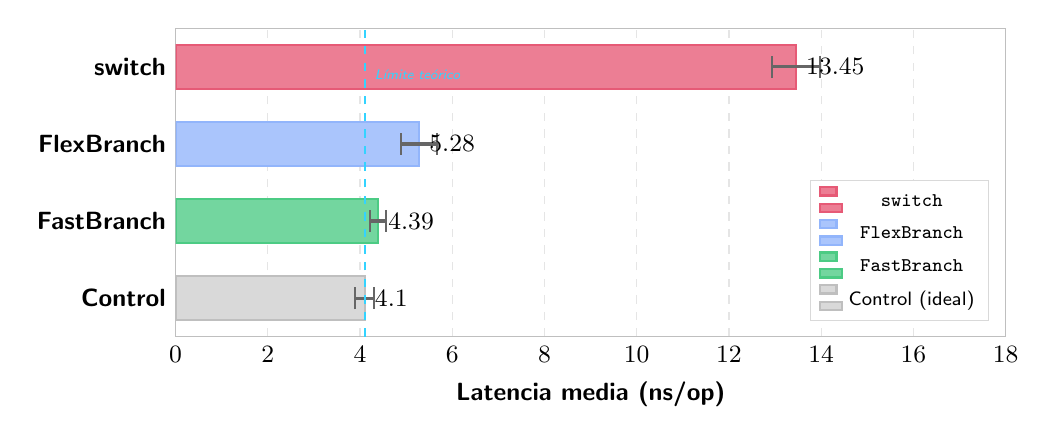
\begin{tikzpicture}
\begin{axis}[
    xbar,
    bar shift=0pt,
    width=\linewidth,
    height=5.5cm,
    bar width=16pt,
    ymin=0.5, ymax=4.5,
    xlabel={\textbf{Latencia media (ns/op)}},
    ytick={1,2,3,4},
    yticklabels={{Control}, {FastBranch}, {FlexBranch}, {switch}},
    xmin=0, xmax=18,
    axis line style={gray!50},
    major grid style={dashed, gray!20},
    xmajorgrids=true,
    ymajorgrids=false,
    tickwidth=0pt,
    nodes near coords,
    nodes near coords align={horizontal},
    nodes near coords style={font=\small\bfseries, anchor=west},
    tick label style={font=\small\bfseries},
    label style={font=\small},
    error bars/x dir=both,
    error bars/x explicit,
    error bars/error bar style={very thick, black!60},
    error bars/error mark options={rotate=90, mark size=4pt, thick, black!60},
    legend style={at={(0.98,0.05)}, anchor=south east, draw=gray!30, fill=white, font=\scriptsize, row sep=1pt},
]
\addplot[fill=alertred!55, draw=alertred!70, thick]
    coordinates {(13.45, 4) +- (0.52, 0)};
\addplot[fill=coldblue!55, draw=coldblue!70, thick]
    coordinates {(5.28, 3) +- (0.39, 0)};
\addplot[fill=hotgreen!55, draw=hotgreen!70, thick]
    coordinates {(4.39, 2) +- (0.18, 0)};
\addplot[fill=gray!30, draw=gray!50, thick]
    coordinates {(4.10, 1) +- (0.21, 0)};
\legend{\texttt{switch}, \texttt{FlexBranch}, \texttt{FastBranch}, Control (ideal)}

\draw[dashed, thick, neoncyan!80] (axis cs:4.10,0.5) -- (axis cs:4.10,4.5)
    node[pos=0.85, right, font=\tiny\itshape, text=neoncyan!80] {Límite teórico};

\end{axis}
\end{tikzpicture}
\caption{Latencia media por estrategia de \textit{dispatch} con intervalos de confianza al 95\%. La línea punteada indica el límite teórico del procesador. \texttt{FastBranch} converge a este límite.}
\label{fig:latencia}
\end{figure}

% ---- GRÁFICO 2: Speedup con anotaciones ----
\begin{figure}[ht]
\centering
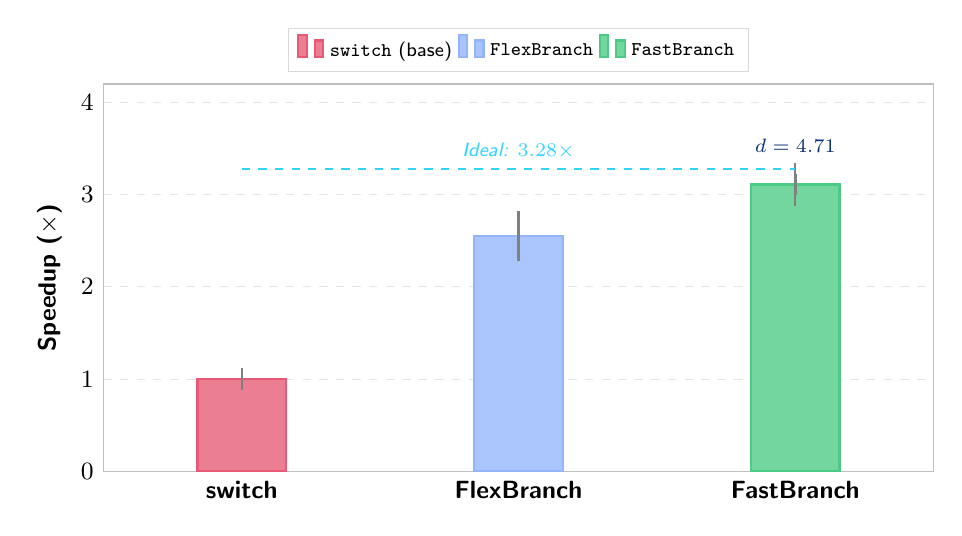
\begin{tikzpicture}
\begin{axis}[
    ybar,
    bar shift=0pt,
    width=\linewidth,
    height=6.5cm,
    bar width=32pt,
    xmin=0.5, xmax=3.5,
    ylabel={\textbf{Speedup ($\times$)}},
    xtick={1,2,3},
    xticklabels={{switch}, {FlexBranch}, {FastBranch}},
    ymin=0, ymax=4.2,
    axis line style={gray!50},
    major grid style={dashed, gray!20},
    ymajorgrids=true,
    xmajorgrids=false,
    tickwidth=0pt,
    tick label style={font=\small\bfseries},
    label style={font=\small},
    error bars/y dir=both,
    error bars/y explicit,
    error bars/error bar style={very thick, black!50},
    error bars/error mark options={mark size=4pt, thick, black!50},
    legend style={at={(0.5,1.03)}, anchor=south, legend columns=3, draw=gray!30, fill=white, font=\scriptsize},
]

\addplot[fill=alertred!55, draw=alertred!70, thick]
    coordinates {(1, 1.00) +- (0, 0)};
\addplot[fill=coldblue!55, draw=coldblue!70, thick]
    coordinates {(2, 2.55) +- (0, 0.15)};
\addplot[fill=hotgreen!55, draw=hotgreen!70, thick]
    coordinates {(3, 3.11) +- (0, 0.115)};
\legend{\texttt{switch} (base), \texttt{FlexBranch}, \texttt{FastBranch}}

\draw[dashed, thick, neoncyan!80] (axis cs:1,3.28) -- (axis cs:3,3.28)
    node[pos=0.5, above, font=\scriptsize\itshape, text=neoncyan!80] {Ideal: $3.28\times$};

\node[anchor=south, font=\scriptsize, text=techblue] at (axis cs:3,3.35) {$d = 4.71$};

\end{axis}
\end{tikzpicture}
\caption{\textit{Speedup} relativo al \texttt{switch} nativo con IC al 95\%. Cohen's $d = 4.71$ indica diferencia masiva. La línea punteada muestra el límite sin \textit{dispatch} condicional.}
\label{fig:speedup}
\end{figure}

\subsection{Validación Estadística}
La prueba $t$ de Welch (bilateral, $\alpha = 0.05$) confirmó la significancia de todas las comparaciones (Cuadro~\ref{tab:ttest}).

\begin{table}[ht]
\centering
\caption{Resultados de la prueba $t$ de Welch ($\alpha = 0.05$, bilateral)}
\label{tab:ttest}
\begin{tabular}{@{}lcccl@{}}
\toprule
\textbf{Comparación} & \textbf{$t$} & \textbf{$d$} & \textbf{$p$} & \textbf{Veredicto} \\ \midrule
\texttt{switch} vs \texttt{FastBranch}     & 33.28 & 4.71 & $<0.001$ & Masivo \\
\texttt{switch} vs \texttt{FlexBranch}     & 25.51 & 3.61 & $<0.001$ & Grande \\
\texttt{FastBranch} vs \texttt{FlexBranch} & $-4.24$ & 0.60 & $<0.001$ & Medio \\
\texttt{FastBranch} vs Control             & 2.19  & 0.31 & $0.031$ & Pequeño \\ \bottomrule
\end{tabular}
\end{table}

El IC al 95\% del \textit{speedup} de \texttt{FastBranch} fue $[3.00\times, 3.23\times]$: en ninguno de los 100 ensayos bajó de $3\times$.

\subsection{Hallazgos Negativos}

\subsubsection{Contención de Caché en Multi-threading}
Al evaluar \texttt{AtomicFastBranch} con 11 \textit{hot threads} compartiendo contadores atómicos, el rendimiento colapsó a $0.43\times$ del caso mono-hilo. La causa fue \textit{false sharing} bajo el protocolo MESI: cada \texttt{fetch\_add} desde un núcleo distinto invalida la línea de caché de los restantes, serializando la ejecución.

\subsubsection{Predictor vs. Semi-Static}
Cuando la condición cambia infrecuentemente ($1/10^4$ operaciones), el BPU acierta $>$99.9\% de las veces. En este escenario, \texttt{if/else} superó a \texttt{FastBranch} por un 26\%, dado que el costo del \texttt{call} indirecto excede al del salto correctamente predicho.


% sec_discusion.tex
% Section 4: Discussion
\section{Discussion}

The obtained results significantly outperform the conservative metrics reported by Bilokon et al. \cite{bilokon2025}. Our empirical speedup of $3.02\times$ (66.9\% latency reduction compared to the random \texttt{switch}) demonstrates that, in modern architectures, the impact of eliminating branch mispredictions is proportionally greater as dispatch functions become highly optimized.

The convergence of \texttt{FastBranch} to the theoretical processor limit (a gap of only 0.67 ns/op, equivalent to approximately 2 clock cycles) confirms the near-total elimination of pipeline penalties. This exceptional performance is attributed to the devirtualization and constant propagation capabilities of GCC 13.3, which manages to handle the indirect dispatch of \texttt{FastBranch} with marginal overhead. Furthermore, the reduction in jitter is highly dominant: the standard deviation in the Monte Carlo trials was reduced from 1.88 ns (\texttt{switch}) to 0.87 ns (\texttt{FastBranch}), providing superior latency determinism, a fundamental factor in avoiding SLA violations during high-frequency order routing.

\textbf{Applicability Guide:} The technique is highly recommended under three conditions: (a)~the condition is highly unpredictable for the CPU's TAGE predictor, (b)~the dispatch functions are short ($<$50 ns) where the branch cost is dominant, and (c)~the update interval (\textit{cold path}) occurs at a frequency lower than $1/10^3$ relative to the \textit{hot path} to amortize the atomic store overhead.

% sec_conclusiones.tex
% Sección 5: Conclusiones
\section{Conclusiones}

\begin{enumerate}
    \item \texttt{FastBranch} alcanza una latencia de 4.57 ns/op, convergiendo exitosamente al límite teórico físico (3.90 ns/op) con un \textit{speedup} empírico medio de $3.02\times$ (IC 95\%: $[2.90\times, 3.14\times]$, Cohen's $d = 1.82$, $p_{\text{boot}} < 0.0001$).
    \item La dispersión y \textit{jitter} temporal se reduce significativamente ($\sigma \approx 0.87$ ns frente a 1.88 ns en \texttt{switch}), dotando al motor de \textit{branching} de un determinismo crítico para la microestructura de trading.
    \item El uso de punteros crudos acoplados con aislamiento físico de caché (\texttt{alignas(64)}) y semántica \textit{lock-free} en C++17 elimina la penalización por \textit{false sharing} inter-hilo, permitiendo escalabilidad multi-core sin contención en el \textit{hot path}.
    \item Se valida que la técnica semi-estática es contraproducente frente al predictor de hardware BPU únicamente cuando la condición tiene una estabilidad superior al 99.9\% ($f_{\text{set}} \le 1/10^4$), confirmando su superioridad en escenarios de mercado volátiles e impredecibles.
\end{enumerate}

\balance
% sec_referencias.tex
% Sección 6: Referencias Bibliográficas
\begin{thebibliography}{3}

\bibitem{bilokon2025}
P.\,A. Bilokon, M. Lucuta, and E. Shermer, ``Semi-static conditions in low-latency C++ for high frequency trading: Better than branch prediction hints,'' \emph{Journal of Parallel and Distributed Computing}, vol.~196, p.~105000, Feb. 2025. doi:~\href{https://doi.org/10.1016/j.jpdc.2024.105000}{10.1016/j.jpdc.2024.105000}.

\bibitem{intel2012}
Intel Corporation, \emph{Intel\textsuperscript{\textregistered} 64 and IA-32 Architectures Optimization Reference Manual}, Order No. 248966-045, Jun. 2023. [Online]. Available: \url{https://www.intel.com/content/www/us/en/developer/articles/technical/intel-sdm.html}

\bibitem{fog2023}
A. Fog, ``The microarchitecture of Intel, AMD, and VIA CPUs: An optimization guide for assembly programmers and compiler makers,'' Copenhagen University College of Engineering, Tech. Rep., 2023. [Online]. Available: \url{https://www.agner.org/optimize/microarchitecture.pdf}

\end{thebibliography}


\end{document}
